\documentclass[11pt,letter]{article}
\usepackage[top=0.70in, bottom=0.8in, left=1.1in, right=1.1in]{geometry}
\usepackage{graphicx} % Required for inserting images
\usepackage{xcolor} 
\definecolor{Accent}{HTML}{bd2b00} 
\usepackage{natbib}
\usepackage{amsmath}
\usepackage{gensymb}
\usepackage{hyperref}
\hypersetup{colorlinks,citecolor = Accent, linkcolor = Accent,urlcolor = Accent, breaklinks=true}
\usepackage{cleveref}
\usepackage[labelfont=bf]{caption}
\bibliographystyle{amnat}

\RequirePackage[labelfont={bf,sf},%
                font={small, sf}]{caption}

\usepackage{lineno}
\renewcommand\linenumberfont{\normalfont\tiny\color{gray}}

\begin{document}

\title{Solstice optimizes thermal growing season\\\emph{Figures}}

\author{Victor Van der Meersch$^{1}$, E. M. Wolkovich$^{1}$}
\date{}
\maketitle 

$^1$ Department of Forest and Conservation Sciences, Faculty of Forestry, University of British Columbia, 2424 Main Mall
Vancouver, BC, Canada, V6T 1Z4. \\

\begin{figure}[h]
	\vspace*{-0.3cm}
	\centering
	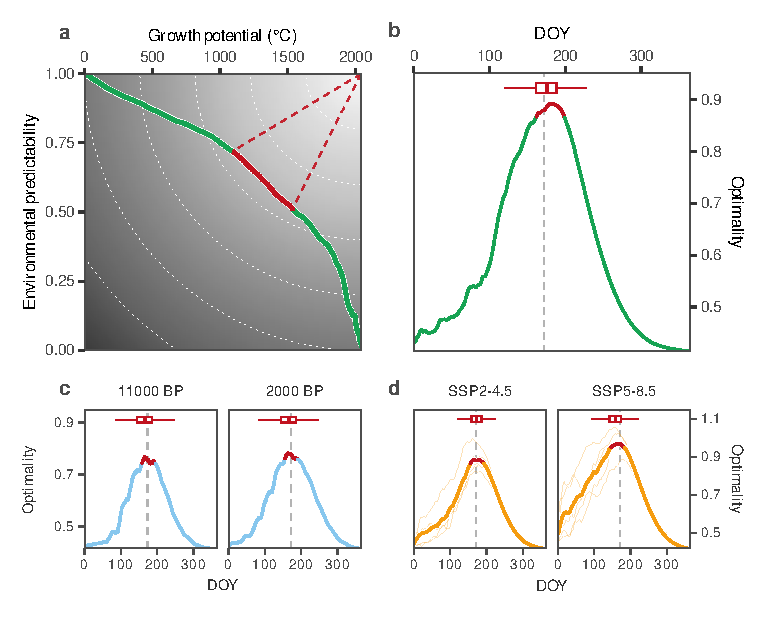
\includegraphics{../../figures/figure1_enriched}
	\vspace*{-0.6cm}
	\vspace*{0.3cm}
	\caption{\textbf{Solstice marks the average optimal trade-off between environmental predictability and growth potential across Europe.} \textbf{(a,b)} represents current climatic conditions (1951-2020), \textbf{(c)} represents past climatic conditions (11000 BP and 2000 BP, where BP stand for "Before Present"), and \textbf{(d)} represents future climatic conditions (for two emission scenarios, SSP2-4.5 and SSP5-8.5). In \textbf{(a)}, environmental predictability measures how well GDD by a given day predicts total yearly GDD ($R^2$ of a linear regression across years), while growth potential represents the remaining GDD from that day onward. In \textbf{(b,c,d)}, optimality is based on the Euclidean distance from the (unattainable) perfect point where both predictability and growth potential are maximized (illustrated by the red dashed lines and the gray gradient in the left panel). The red sections of the curves represent days where optimality falls within the 90th percentile (i.e. top 10\% most optimal days). GDD range was defined between 5\degree C and 35\degree C (see \Cref{fig:altgdd} for 0-40\degree C). BP stand for "Before Present" (i.e. 1950).} 
	\label{fig:globaloptimality}
\end{figure}

\clearpage

\begin{figure}[]
	 \centering
	\hspace*{-1.2cm}
	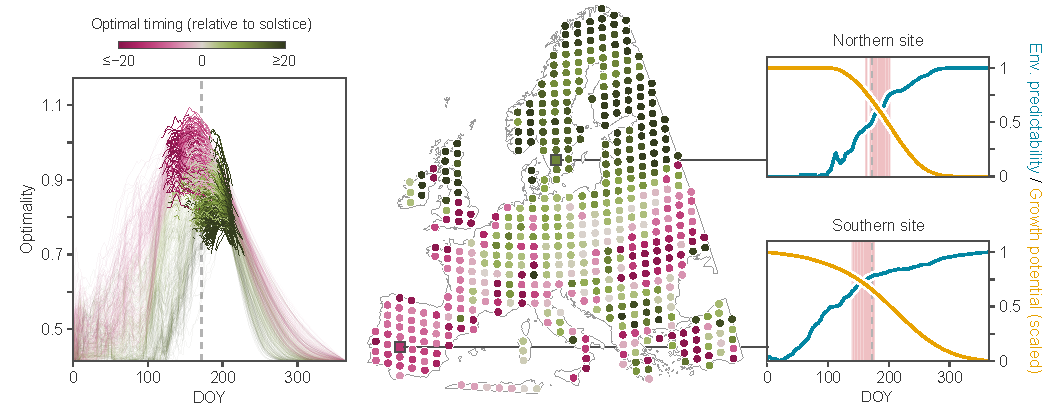
\includegraphics{../../figures/local_optimality_alt}
	\vspace*{-0.9cm} %emw19Jan -- I tried to spell out a little more this difference in optimal for the average versus for each site.
	\vspace*{0.3cm}
	\caption{\textbf{Average optimal timing (\Cref{fig:globaloptimality}) hides variation in optimal timing across the different climatic conditions of Europe (1951-2020).} On the left panel, each curve shows the optimality for a given site. Sites are sampled on a regular grid across Europe, as shown on the central map. Colors indicate the timing---relative to the solstice---of the median optimal day. The two panels on the right show the trade-off between environmental predictability and growth potential (scaled to $[0,1]$) for two different sites. Days considered as optimal are highlighted in red.}
	\label{fig:localoptimality}
\end{figure}

\clearpage

%\begin{figure}
%	\centering
%	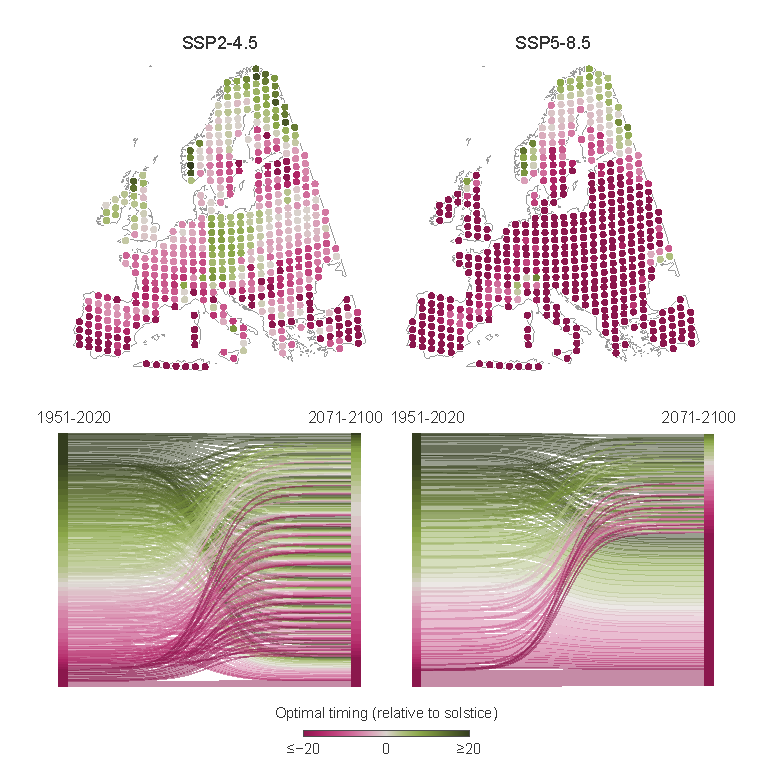
\includegraphics[scale = 1]{../../figures/supp/local_optimality_future.pdf}
%	\vspace*{0.3cm}
%	\caption{\textbf{Average optimal timing (\Cref{fig:globaloptimality}) hides variation in optimal timing across the different future climatic conditions of Europe (2071-2100).} On the top panel, sites are sampled on a regular grid across Europe. On the bottom panel, Sankey diagrams show the proportional flow of (site-specific) optimal timing from 1951-2020 to 2071-2100. Colors indicate the timing—relative to the solstice—of the median optimal day.}
%	\label{fig:futurelocal}
%\end{figure}

\end{document}
